

\begin{multicols}{2}

% Il faudrait créer une variable python ["le double","le triple","le quadruple","le quintuple","la moitié",le "tiers","le quart", "le cinquième", "le dixième"] et l'utiliser dans l'exercice ainsi qu'une variable ["la somme", "la différence", "le produit", "le quotient"]
%\exo{}
%
%Traduire par une expression littérale : 
%\begin{enumerate}
%	\item le double de $z$
%	\item le triple de $z$
%	\item la moitié de $z$
%	\item le produit de 7 par $z$
%	\item la somme du produit de 5 par $z$ et du\\ double de $z$
%	\item le double de la somme de 5 et $z$
%\end{enumerate}

%% for i in range(0,61,20) 
\exo{ - Version <<i / 20 +1>>}
Quel résultat donne chacun de ces 3 programmes de calculs lorsqu'on prend $x$ comme nombre de départ ?	

\begin{center}
\fcolorbox{black}{gray!30}{
\begin{minipage}{0.7\linewidth}
Programme 1 : 
\begin{itemize}
	\item Multiplier par <<nZ[1+i]>>
	\item Ajouter <<nZ[2+i]>>
\end{itemize}
\end{minipage}
}

\medskip
\fcolorbox{black}{gray!30}{
\begin{minipage}{0.7\linewidth}
Programme 2 : 
\begin{itemize}
	\item Soustraire <<nZ[3+i]>>
	\item Multiplier par <<nZ[4+i]>>
\end{itemize}
\end{minipage}
}

\medskip
\fcolorbox{black}{gray!30}{
\begin{minipage}{0.7\linewidth}
Programme 3 : 
\begin{itemize}
	\item Multiplier par <<nZ[5+i]>>
	\item Soustraire <<nZ[6+i]>>
	\item Prendre le double
\end{itemize}
\end{minipage}
}
\end{center}
%% endfor

%% for i in range(0,61,20) 
\exo{ - Version <<i / 20 +1>>}

Simplifier les expressions suivantes.

\begin{multicols}{2}
$A=<<n[1+i]>> x <<terme(m[1+i])>> x$\\
$B=x\times <<facteur(mZ[2+i])>> \times x$\\
$C=<<nZ[7+i]>>\times x <<terme(nZ[8+i])>>\times x$\\
$D=<<nZ[7+i]>>\times x\times <<facteur(nZ[8+i])>>\times x$\\
$E=<<nZ[9+i]>> \times x<<terme(nZ[10+i])>>\times <<facteur(nZ[11+i])>> <<terme(nZ[12+i])>> x$\\
$F=<<nZ[13+i]>> \times (<<nZ[14+i]>>y <<terme(nZ[15+i])>>)$\\
$G=<<N2[1+i]>> a\times  a+a\times <<N2[2+i]>>+a\times <<N3[1+i]>>$\\
$H= <<nZ[17+i]>>\times x <<terme(nZ[18+i])>>x$
\end{multicols}
%% endfor

%% for i in range(0,61,20) 

%
%\exo{}
%
%Calculer les expressions suivantes pour $x=<<n[19]>>$.
%
%\begin{tasks}[counter-format = {tsk[1].},label-format={\bfseries}](3)
%	\task $<<nZ[20]>> x$ 
%	\task $x^2$
%	\task $<<mZ[20]>>x <<terme(mZ[19])>> $
%	\task $ <<mZ[18]>> (<<mZ[16]>> x <<terme(mZ[16])>>)$
%	\task $ <<mZ[15]>>  <<terme(mZ[14])>> x$
%	\task $x^3$
%\end{tasks}

\exo{ - Version <<i / 20 +1>>}

Développer et réduire les expressions suivantes.

\begin{multicols}{2}
$A=  <<mZ[12+i]>> (x  <<terme(mZ[13+i])>>)$\\
$B= <<mZ[11+i]>> ( <<mZ[10+i]>> x    <<terme(mZ[9+i])>>)$\\
$C=y( <<mZ[7+i]>>  <<terme(mZ[8+i])>> y)$\\
$D= <<mZ[6+i]>>  t(  <<mZ[5+i]>> t <<terme(mZ[4+i])>>)$
\end{multicols}

%% endfor

%% for i in range(0,61,20) 
\exo{ - Version <<i / 20 +1>>}

Factoriser les expressions suivantes.

\begin{multicols}{2}
$E=  <<N[5+i] * n[1+i]>> x  <<terme(S[1+i] * n[1+i])>>$\\
$F=  <<S[6+i] *n[6+i] * n[2+i]>> x  <<terme(S[2+i] * n[2+i])>> x$\\
$G=  <<S[7+i] *N[7+i] * n[3+i]>> x  <<terme(S[3+i] * n[3+i])>> x^2$\\
$H=  <<S[8+i] *n[8+i] >> x^2  <<terme(S[4+i] *n[4+i] )>> x^2$
\end{multicols}

%% endfor

\raggedcolumns
\end{multicols}

\exon{}

\begin{minipage}{0.4\linewidth}
	\begin{center}
	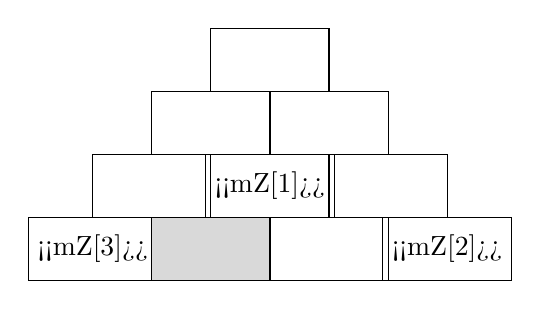
\begin{tikzpicture}
		\tikzstyle{brique}=[minimum width=1.5cm, minimum height=0.8cm,draw]
		\tikzstyle{brique_grise}=[minimum width=1.5cm, minimum height=0.8cm,draw,fill=gray!30]
		\node[brique] at (0,0) {  <<mZ[3]>> }; % gauche
		\node[brique_grise] at (1.5,0) {};
		\node[brique] at (3,0) {};
		\node[brique] at (4.5,0) { <<mZ[2]>> };  % droite
		\node[brique] at (.75,.8) {};
		\node[brique] at (2.25,.8) {  <<mZ[1]>> };  % milieu bas
		\node[brique] at (3.75,.8) {};
		\node[brique] at (1.5,1.6) {};
		\node[brique] at (3,1.6) {};
		\node[brique] at (2.25,2.4) {};
	\end{tikzpicture} 	
\end{center}
\end{minipage}
\begin{minipage}{0.6\linewidth}
Pour compléter cette pyramide, le nombre situé dans une case est la somme des deux nombres situés en dessous de lui.

\begin{enumerate}
	\item Compléter cette pyramide en mettant un nombre au choix dans la case grise.
	\item Benjamin affirme : \og{} Quel que soit le nombre que je place dans la case grise, je trouve toujours <<mZ[3] + mZ[2] + 3*mZ[1]>> dans la case la plus haute. \fg{}. Est-ce vrai ou faux ? Démontrer le.
\end{enumerate}
\end{minipage}


%\exon{}
%
%
%\begin{center}
%\fcolorbox{black}{gray!30}{
%\begin{minipage}{0.5\linewidth}
%\begin{itemize}
%	\item Multiplier par <<nZ[41]>>
%	\item Enlever <<nZ[41]>>
%	\item Multiplier par <<nZ[41]>>
%	\item Ajouter <<nZ[41]>>
%	\item Enlever quatre fois le nombre de départ
%\end{itemize}
%\end{minipage}
%}
%\end{center}
%
%\begin{enumerate}
%	\item Après avoir lu ce programme, Benjamin dit : \og{} C'est complètement inutile de faire toutes ces étapes, en un seul calcul je trouve le résultat. \fg{}.\\
%Démontrer que Benjamin a raison et expliquer la seule étape nécessaire.
%	\item Quel nombre de départ faut-il choisir pour obtenir 13 comme résultat avec ce programme de calcul ?
%\end{enumerate}
%
%\exon{}
%
%\begin{tabularx}{\linewidth}{*{4}{>{\centering\arraybackslash}X}}
%\begin{tikzpicture}
%	\tikzstyle{carré}=[minimum width=.5cm, minimum height=.5cm,draw]
%	\node[carré] at (0,0) {};
%\end{tikzpicture}
%&
%\begin{tikzpicture}
%	\tikzstyle{carré}=[minimum width=.5cm, minimum height=.5cm,draw]
%	\node[carré] at (0,0) {};
%	\node[carré] at (-.5,0) {};
%	\node[carré] at (.5,0) {};
%	\node[carré] at (0,.5) {};
%\end{tikzpicture}
%&
%\begin{tikzpicture}
%	\tikzstyle{carré}=[minimum width=.5cm, minimum height=.5cm,draw]
%	\node[carré] at (0,0) {};
%	\node[carré] at (-.5,0) {};
%	\node[carré] at (-1,0) {};
%	\node[carré] at (.5,0) {};
%	\node[carré] at (1,0) {};
%	\node[carré] at (0,.5) {};
%	\node[carré] at (0,1) {};
%\end{tikzpicture}
%&
%\begin{tikzpicture}
%	\tikzstyle{carré}=[minimum width=.5cm, minimum height=.5cm,draw]
%	\node[carré] at (0,0) {};
%	\node[carré] at (-.5,0) {};
%	\node[carré] at (-1,0) {};
%	\node[carré] at (-1.5,0) {};
%	\node[carré] at (.5,0) {};
%	\node[carré] at (1,0) {};
%	\node[carré] at (1.5,0) {};
%	\node[carré] at (0,.5) {};
%	\node[carré] at (0,1) {};
%	\node[carré] at (0,1.5) {};
%\end{tikzpicture}
%\\[-.1cm]
%\textbf{Étape 1} & \textbf{Étape 2} & \textbf{Étape 3} & \textbf{Étape 4}\\
%\end{tabularx}
%
%\bigskip
%\begin{enumerate}
%    \item Combien faut-il de carrés à l'étape 5 ?
%    \item Proposer une formule permettant de calculer le nombre de
%      carrés nécessaires pour l'étape $N$.
%    \item Combien faut-il de carrés à l'étape 1~000 ?
%\end{enumerate}


%	
%
%
%
%\setcounter{exo}{0}
%\vfill
%\begin{correction}
%\begin{multicols}{2}

%
%\exo{}
%
%Programme 1 : $<<nZ[1]>> x <<terme(nZ[2])>>$\\
%Programme 2 : $(x <<terme(nZ[3])>>)\times <<facteur(nZ[4])>>= <<nZ[4]>>  x  << terme( nZ[4] * nZ[3] ) >> $\\
%Programme 3 : $( <<nZ[5]>> x <<terme(nZ[6])>> )\times 2= <<2* nZ[5]>> x <<terme(nZ[6])>>$
%
%\exo{}
%
%
%\begin{multicols}{2}
%$A=<<S[1]+1>> x$\\
%$B=<<S[2]>>x^2$\\
%$C=(<<nZ[7]>> <<terme(nZ[8])>>)\times x = <<nZ[7] + nZ[8]>>  x$\\
%$D=<<nZ[7]>> \times <<facteur(nZ[8])>>\times x^2 = <<nZ[7] * nZ[8]>>\times x^2$\\
%$E=<<nZ[9]>> \times x <<terme(nZ[10])>>\times <<facteur(nZ[11])>> <<terme(nZ[12])>> x$\\
%$F=<<nZ[13]>> \times (y\times <<facteur(nZ[14])>> <<terme(nZ[15])>> \times <<facteur(nZ[16])>>)$\\
%$G=<<N2[1]>> a\times  a+a\times <<N2[2]>>+a\times <<N3[1]>>$\\
%$H= <<nZ[17]>>\times x <<terme(nZ[18])>>$
%\end{multicols}
%
%
%
%\exo{}
%
%
%\begin{tasks}[counter-format = {tsk[1].},label-format={\bfseries}](3)
%	\task $2\times3=6$ 
%	\task $3^2=9$
%	\task $2\times3-5=1$
%	\task $3\times13=39$
%	\task $2-3=-1$
%	\task $3^3=27$
%\end{tasks}
%
%\exo{}
%
%
%\begin{multicols}{2}
%$A=3x+15$\\
%$B=10x-15$\\
%$C=3y+5y^2$\\
%$D=6t^2-12t$
%\end{multicols}
%
%\end{multicols}
%
%	
%
%
%	
%\end{correction}
